% UCL Thesis LaTeX Template
% 
% This is a template/skeleton for PhD/MPhil/MRes theses.
%
% It uses a rather split-up file structure because this tends to
%  work well for large, complex documents.
% We suggest using one file per chapter, but you may wish to use more
%  or fewer separate files than that.
% We've also separated out various bits of configuration into their
%  own files, to keep everything neat.
% Note that the \input command just streams in whatever file you give
%  it, while the \include command adds a page break, and does some
%  extra organisation to make compilation faster. Note that you can't
%  use \include inside an \include-d file.
% We suggest using \input for settings and configuration files that
%  you always want to use, and \include for each section of content.
% If you do that, it also means you can use the \includeonly statement
%  to only compile up the section you're currently interested in.
% You might also want to put figures into their own files to be \input.

% For more information on \input and \include, see:
%  http://tex.stackexchange.com/questions/246/when-should-i-use-input-vs-include


% Formatting rules for theses are here: 
%  http://www.ucl.ac.uk/current-students/research_degrees/thesis_formatting
% Binding and submitting guidelines are here:
%  http://www.ucl.ac.uk/current-students/research_degrees/thesis_binding_submission

% This package goes first and foremost, because it checks all 
%  your syntax for mistakes and some old-fashioned LaTeX commands.
% Note that normally you should load your documentclass before 
%  packages, because some packages change behaviour based on
%  your document settings.
% Also, for those confused by the RequirePackage here vs usepackage
%  elsewhere, usepackage cannot be used before the documentclass
%  command, while RequirePackage can. That's the only functional
%  difference.
\RequirePackage[l2tabu, orthodox]{nag}


% ------ Main document class specification ------
% The draft option here prevents images being inserted,
%  and adds chunky black bars to boxes that are exceeding 
%  the page width (to show that they are).
% The oneside option can optionally be replaced by twoside if
%  you intend to print double-sided. Note that this is
%  *specifically permitted* by the UCL thesis formatting
%  guidelines.
%
% Valid options in terms of type are:
%  phd
%  mres
%  mphil
%\documentclass[12pt,phd,draft,a4paper,oneside]{ucl_thesis}
\documentclass[12pt,mres,a4paper,oneside]{ucl_thesis}


% Package configuration:
%  LaTeX uses "packages" to add extra commands and features.
%  There are quite a few useful ones, so we've put them in a 
%   separate file.
% -------- Packages --------


%%%%%%%%%%%%%%%%%%%%%%%%%%%%%%%%%%%%%%%%%%%%%%%%%%%%%%%%%%%%%%%
%MY OWN PACKAGES
\usepackage{datetime} %put those 2 to display the full date on the first page
\newdateformat{monthyeardate}{\monthname[\THEMONTH], \THEYEAR} %put those 2 to display the full date

\usepackage{titlesec}% to make the title of each chapter appear better
\usepackage{cite}%for citing
\usepackage{longtable} %for long tables
\usepackage{color}%for table
\usepackage[table,xcdraw]{xcolor} %for table



\usepackage[T1]{fontenc}
\usepackage{graphics}
\usepackage{rotating, graphicx}
\usepackage{booktabs}



%%%%%%%%%%%%%%%%%%%%%%%%%%%%%%%%%%%%%%%%%%%%%%%%%%%%%%%%%%%%%%%

% This package just gives you a quick way to dump in some sample text.
% You can remove it -- it's just here for the examples.
\usepackage{blindtext}

% This package means empty pages (pages with no text) won't get stuff
%  like chapter names at the top of the page. It's mostly cosmetic.
\usepackage{emptypage}

% The graphicx package adds the \includegraphics command,
%  which is your basic command for adding a picture.
\usepackage{graphicx}

% This command is provided by the graphicx package, and 
%  controls the default dpi resolution of images you use.
%  72 is the default, but 300 is more normal, and 600 is
%  as good as you can expect to be able to get on normal paper.
\pdfimageresolution=300


% The float package improves LaTeX's handling of floats,
%  and also adds the option to *force* LaTeX to put the float
%  HERE, with the [H] option to the float environment.
\usepackage{float}

% The amsmath package enhances the various ways of including
%  maths, including adding the align environment for aligned
%  equations.
\usepackage{amsmath}

% Use these two packages together -- they define symbols
%  for e.g. units that you can use in both text and math mode.
\usepackage{gensymb}
\usepackage{textcomp}
% You may also want the units package for making little
%  fractions for unit specifications.
%\usepackage{units}


% The setspace package lets you use 1.5-sized or double line spacing.
\usepackage{setspace}
\setstretch{1.5}

% That just does body text -- if you want to expand *everything*,
%  including footnotes and tables, use this instead:
%\renewcommand{\baselinestretch}{1.5}


% PGFPlots is either a really clunky or really good way to add graphs
%  into your document, depending on your point of view.
% There's waaaaay too much information on using this to cover here,
%  so, you might want to start here:
%   http://pgfplots.sourceforge.net/
%  or here:
%   http://pgfplots.sourceforge.net/pgfplots.pdf
%\usepackage{pgfplots}
%\pgfplotsset{compat=1.3} % <- this fixed axis labels in the version I was using

% PGFPlotsTable can help you make tables a little more easily than
%  usual in LaTeX.
% If you're going to have to paste data in a lot, I'd suggest using it.
%  You might want to start with the manual, here:
%  http://pgfplots.sourceforge.net/pgfplotstable.pdf
%\usepackage{pgfplotstable}

% These settings are also recommended for using with pgfplotstable.
%\pgfplotstableset{
%	% these columns/<colname>/.style={<options>} things define a style
%	% which applies to <colname> only.
%	empty cells with={--}, % replace empty cells with '--'
%	every head row/.style={before row=\toprule,after row=\midrule},
%	every last row/.style={after row=\bottomrule}
%}


% The mhchem package provides chemistry formula typesetting commands
%  e.g. \ce{H2O}
%\usepackage[version=3]{mhchem}

% And the chemfig package gives a weird command for adding Lewis 
%  diagrams, for e.g. organic molecules
%\usepackage{chemfig}

% The linenumbers command from the lineno package adds line numbers
%  alongside your text that can be useful for discussing edits 
%  in drafts.
% Remove or comment out the command for proper versions.
%\usepackage[modulo]{lineno}
% \linenumbers 


% Alternatively, you can use the ifdraft package to let you add
%  commands that will only be used in draft versions
%\usepackage{ifdraft}

% For example, the following adds a watermark if the draft mode is on.
%\ifdraft{
%  \usepackage{draftwatermark}
%  \SetWatermarkText{\shortstack{\textsc{Draft Mode}\\ \strut \\ \strut \\ \strut}}
%  \SetWatermarkScale{0.5}
%  \SetWatermarkAngle{90}
%}


% The multirow package adds the option to make cells span 
%  rows in tables.
\usepackage{multirow}


% Subfig allows you to create figures within figures, to, for example,
%  make a single figure with 4 individually labeled and referenceable
%  sub-figures.
% It's quite fiddly to use, so check the documentation.
%\usepackage{subfig}

% The natbib package allows book-type citations commonly used in
%  longer works, and less commonly in science articles (IME).
% e.g. (Saucer et al., 1993) rather than [1]
% More details are here: http://merkel.zoneo.net/Latex/natbib.php
%\usepackage{natbib}

% The bibentry package (along with the \nobibliography* command)
%  allows putting full reference lines inline.
%  See: 
%   http://tex.stackexchange.com/questions/2905/how-can-i-list-references-from-bibtex-file-in-line-with-commentary
\usepackage{bibentry} 

% The isorot package allows you to put things sideways 
%  (or indeed, at any angle) on a page.
% This can be useful for wide graphs or other figures.
%\usepackage{isorot}

% The caption package adds more options for caption formatting.
% This set-up makes hanging labels, makes the caption text smaller
%  than the body text, and makes the label bold.
% Highly recommended.
\usepackage[format=hang,font=small,labelfont=bf]{caption}

% If you're getting into defining your own commands, you might want
%  to check out the etoolbox package -- it defines a few commands
%  that can make it easier to make commands robust.
\usepackage{etoolbox}


% Sets up links within your document, for e.g. contents page entries
%  and references, and also PDF metadata.
% You should edit this!!!!!!!!!
%%
%% This file uses the hyperref package to make your thesis have metadata embedded in the PDF, 
%%  and also adds links to be able to click on references and contents page entries to go to 
%%  the pages.
%%

% Some hacks are necessary to make bibentry and hyperref play nicely.
% See: http://tex.stackexchange.com/questions/65348/clash-between-bibentry-and-hyperref-with-bibstyle-elsart-harv
\usepackage{bibentry}

\makeatletter\let\saved@bibitem\@bibitem\makeatother
\usepackage[driverfallback=dvipdfm]{hyperref}%and inserted this one
%\usepackage[pdftex,hidelinks]{hyperref} %that was by default but had errors compiling with Latex (not PDFLatex), so i commented it out
\makeatletter\let\@bibitem\saved@bibitem\makeatother
\makeatletter
\AtBeginDocument{
    \hypersetup{
        pdfsubject={Thesis Subject},
        pdfkeywords={Thesis Keywords},
        pdfauthor={Author},
        pdftitle={Title},
    }
}
\makeatother
    


% And then some settings in separate files.
% These settings are from:
%  http://mintaka.sdsu.edu/GF/bibliog/latex/floats.html

% They give LaTeX more options on where to put your figures, and may
%  mean that fewer of your figures end up at the tops of pages far
%  away from the thing they're related to.

% Alters some LaTeX defaults for better treatment of figures:
% See p.105 of "TeX Unbound" for suggested values.
% See pp. 199-200 of Lamport's "LaTeX" book for details.

%   General parameters, for ALL pages:
\renewcommand{\topfraction}{0.9}	% max fraction of floats at top
\renewcommand{\bottomfraction}{0.8}	% max fraction of floats at bottom

%   Parameters for TEXT pages (not float pages):
\setcounter{topnumber}{2}
\setcounter{bottomnumber}{2}
\setcounter{totalnumber}{4}     % 2 may work better
\setcounter{dbltopnumber}{2}    % for 2-column pages
\renewcommand{\dbltopfraction}{0.9}	% fit big float above 2-col. text
\renewcommand{\textfraction}{0.07}	% allow minimal text w. figs

%   Parameters for FLOAT pages (not text pages):
\renewcommand{\floatpagefraction}{0.7}	% require fuller float pages
% N.B.: floatpagefraction MUST be less than topfraction !!
\renewcommand{\dblfloatpagefraction}{0.7}	% require fuller float pages

% remember to use [htp] or [htpb] for placement,
% e.g. 
%  \begin{figure}[htp]
%   ...
%  \end{figure} % For things like figures and tables
% Title Settings. This is just setting it, not printing them. It is printed in the preemble.
\setcounter{secnumdepth}{3}%taken from SE
\setcounter{tocdepth}{3}%taken from SE

\title{Sensor fusion for training doctors}
\author{Dimitrios Selalmazidis}
\department{Department of Computer Science}
\titleformat{\chapter}[display] {\normalfont\Huge\bfseries}{\chaptertitlename\ \thechapter}{0pt}{\Huge}
\titlespacing{\chapter}{0cm}{0 cm}{1.5cm} %first is gap from left, second is from the top, and third is from the bottom
%\titlespacing{\chapter}{0pt}{-40pt}{10pt}



\AtEndDocument{%
\begin{flushright}
    \small This document was set in the Times Roman typeface using \LaTeX\ and Bib\TeX , composed with a text editor. 
\end{flushright}}


\lstdefinestyle{sharpc}{language=[Sharp]C, frame=lr, rulecolor=\color{blue!80!black}}% specifically for c sharp code

\begin{document}

\raggedright

\nobibliography*
% This is a dumb trick that works with the bibentry package to let
%  you put bibliography entries whereever you like.
% I used this to put references to papers a chapter's work was 
%  published in at the end of that chapter.
% For more information, see: http://stefaanlippens.net/bibentry

% If you haven't finished making your full BibTex file yet, you
%  might find this useful -- it'll just replace all your
%  citations with little superscript notes.
% Uncomment to use.
%\renewcommand{\cite}[1]{\emph{\textsuperscript{[#1]}}}

% At last, content! Remember filenames are case-sensitive and 
%  *must not* include spaces.
%the preemble includes the 


%this is the preemble. It includes the title, the decleration, the abstract, the acknowledgements, table of contents, list of figures and list of tables
\maketitle
%\makedeclaration
\vspace{\fill}
\begin{abstract} % 300 word limit
My research is about stuff.

It begins with a study of some stuff, and then some other stuff and things.

There is a 300-word limit on your abstract.
\end{abstract}
\vspace{\fill}

\begin{acknowledgements}
Acknowledge all the things!
\end{acknowledgements}

\setcounter{tocdepth}{2} 
% Setting this higher means you get contents entries for
%  more minor section headers.

\tableofcontents
\listoffigures
\listoftables


\pagenumbering{arabic} 
\setcounter{page}{1}
\chapter{Introduction}% should be around 2-4 pages
\label{chapterlabel1} %this is chapter label

Some stuff about things.\cite{example-citation} Some more things. 

Inline citation: \bibentry{example-citation}


% This just dumps some pseudolatin in so you can see some text in place.
\blindtext
\blindtext
\blindtext
\blindtext
\blindtext



\chapter{Background Information and related work}
\label{chapter2label}

\section{Outline of information sources used for development}
\label{outline_information_for_development}

Jordan De souza


\section{Literature Review}
\label{literature_review}








\section{Aims and Project Scope}
\label{aims_project_scope}

elizabeth

\section{Project Timeline}
\label{project_timeline}

elizabeth



\section{Work Balancing and Process Framework}

elizabeth





\chapter{Requirements and Analysis}
\label{chapterlabel3}


This Chapter establishes the requirements and analysis for this work. The developments of the requirements is a crucial part of the analysis for almost all of the software development projects.

This phase is extremely useful, as for it's flexibility - if things that are unnecessarily complicated are discovered, or are less important to the client, they can be disregarded  or their importance could be downgraded so that they take less time. This is significantly useful for the implementation phase. This is also the easiest time to communicate with the client, while the subject matter is strictly textual, so any major issues or changes to the specifications can be established here.


\section{Problem Statement}
\label{problem_st}

Design a web based application, that allows surgeons to register an operation, upload and view all the extracted data coming from the operating theatre's sensors.


\section{Software Requirement Listing and Prioritization}
\label{sec:softreqlistandprior} 

This stage facilitates a comprehensive understanding of the client's needs and to appreciate the potential complexity of the system. Subsection \ref{sub:functional_req} details the functional requirements of our system.  Functional requirements show the behaviours of the system - what the client wants the system to do.  Subsection \ref{sub:non_functional_req} goes through the non-functional requirements, which affect the system's performance . 
The requirements were gathered through discussion with the client and also by continually iterating over what the application would be used for, so that additional focus should be given on the user needs.


 As mentioned, the requirements have been divided into functional and non-functional \cite{Software_Requirements}. They have also been prioritised according to the MoSCoW prioritisation technique\cite{cleggbarker1994}, in order to guide the progress of the project and to ensure that a base-level application that achieved the goals of the project. The MoSCoW priorities refer to the order of design and development in order. Must have, Should Have, Could Have, and Won't have requirements.




\subsection{Functional Requirements}
\label{sub:functional_req}

\newcounter{magicrownumbers}
\newcommand\rownumber{\stepcounter{magicrownumbers}\arabic{magicrownumbers}}
{
\footnotesize
%\centering
\begin{longtable}{|p{0.5cm}|p{13cm}p{1.3cm}|}

\rowcolor[HTML]{000000}
{\color[HTML]{FFFFFF} \textbf{ID}} & {\color[HTML]{FFFFFF} \textbf{Functional Requirements}}  & {\color[HTML]{FFFFFF} \textbf{Priority}} \\ \hline \endhead
\multicolumn{3}{|c|}{\textbf{Uploading a new Operation}} \\ \hline
\rownumber & The platform shall support a User Interface that will allow the user to register a new operation &Must  \\ \hline
\rownumber & The platform shall be able to take as input from the user, the hospital that the operation took place &Must  \\ \hline
\rownumber & The platform shall be able to take as input from the user, the operating room that the operation took place &Must  \\ \hline
\rownumber & The platform shall be able to take as input from the user, all the staff that participated in the operation &Must  \\ \hline
\rownumber & The platform shall be able to take as input from the user, the type of the operation (Neurosurgery, Hand surgery, Paediatric surgery etc.) &Must  \\ \hline
\rownumber & The platform shall be able to take as input from the user, the specific patient that has undergone the surgery including the patients unique identification number &Must  \\ \hline
\rownumber & The platform shall be able to take as input from the user, all the video files that were produced during the operation &Must  \\ \hline
\rownumber & The platform shall be able to take as input from the user, all the audio files that were produced during the operation &Must  \\ \hline
\rownumber & The platform shall be able to take as input from the user, the file extracted from the patient's monitoring system &Should  \\ \hline
\rownumber & The platform shall be able to record, store and distinguish data from different operating theatres &Must  \\ \hline
\rownumber & The platform shall be able to store all the input data from the user to a relational database &Must  \\ \hline
\rownumber & The platform shall store all the data coming from an operation in a way that all relevant data of the operation could be extracted &Must  \\ \hline
\rownumber & The platform shall be able to process the video, audio and patients monitoring files uploaded from the user &Must  \\ \hline
\rownumber & The platform shall be able to extract all the meta-data from the input files (encoded date, size, duration, file type, file name, full file path) &Must  \\ \hline
\rownumber & The platform shall be able to store the meta-data extracted from the input files, to the relational database &Must  \\ \hline
\rownumber & The platform shall be able to store the input files to an Azure Blob Storage Account &Must  \\ \hline
\rownumber & The platform shall be able to link the files stored in the Azure Blob Storage with the relative operation identification number stored in the relational database &Must  \\ \hline


\multicolumn{3}{|c|}{\textbf{Searching for an Operation}} \\ \hline
\rownumber & The platform shall support searching capabilities; the user of the platform must be able to search an operation/procedure using relevant criteria  &Must  \\ \hline
\rownumber & The platform shall support filtering capabilities where the user can apply specific filters for an operation (hospital name, operating room number, from/to date, doctors name, patient's name, type) &Must  \\ \hline

\multicolumn{3}{|c|}{\textbf{Details of an Operation}} \\ \hline
\rownumber & The platform shall be able to display a specific page where the user can see all the relative information and details of a specific operation &Must  \\ \hline
\rownumber & The platform shall be able to retrieve all the relevant data from the operation (video data, microphone data, patient's monitoring system data etc.) &Must  \\ \hline
\rownumber & The platform shall be able to convert the data coming from the different sensors to easily handled format ( e.g. convert a variety of video input to .avi) &Could  \\ \hline
\rownumber & The platform shall support the capability of switching to a specific moment in time and view all the recorded data at that moment &Could  \\ \hline
\rownumber & The platform shall be able to present to the user all the data recorded from the sensors at the same time. For example it could be able to view the panoramic camera, the light camera, the heart rate, the temperature of the room through the common factor of time. &Could  \\ \hline
\rownumber & The platform shall provide the media files' URL to the user in order for the user to have access to them and re-play them &Must  \\ \hline

\caption[Functional Requirements]{Functional Requirements} % needs to go inside longtable environment
\label{functionalreq}
\end{longtable}
}

\subsection{Non Functional Requirements}
\label{sub:non_functional_req}

{\footnotesize
%\newcommand\rownumber{\stepcounter{magicrownumbers}\arabic{magicrownumbers}}
%\centering
\begin{longtable}{|p{0.5cm}|p{13cm}p{1.3cm}|}

\rowcolor[HTML]{000000}
{\color[HTML]{FFFFFF} \textbf{ID}} &{\color[HTML]{FFFFFF} \textbf{Non-Functional Requirements}}  & {\color[HTML]{FFFFFF} \textbf{Priority}} \\ \hline \endhead
\rownumber & The platform shall use web browser as its user interface & Must \\ \hline
\rownumber & The platform shall support new sensor adding or should require minimal work for new, unknown sensor adding & Should \\ \hline
\rownumber & The platform shall store all the input data in a way that they could be extracted for machine learning purposes (machine learn-able data) & Must \\ \hline
\rownumber & The platform shall be independent of the format of the input data & Should  \\ \hline
\rownumber & The platform shall work on a wide range of operating conditions (screen size, internet connection, performance) & Must \\ \hline
\rownumber & The platform shall be a C\# web application with an MySQL Database & Should \\ \hline
\rownumber & The System shall present search results within 5 seconds & Should \\ \hline

\caption[Non-Functional Requirements]{Non-Functional Requirements} % needs to go inside longtable environment
\label{nonfunctionalreq}
\end{longtable}
}


\section{Domain Modelling}
\label{sec:DomainModelling}
The domain model looks to identify the objects of a system in terms of the requirements. It provides a conceptual real-world view of the system and enables a simplistic overview of the system's functionalities in terms of the problem domain entities \cite{DomainModeling}.
More specifically, the classes were derived from the requirements list where the identified entities were marked in bold. Therefore, it is now possible to create a simple draft domain model from these entities. Furthermore, objects which were deemed redundant from this iteration were also
discarded to refine the list of entities. This initial model was then revised and additional domain objects were
added. Similar to previous analyses, the domain model is therefore the result of an iterative process.

Following the refinement process, using the identified entities of the requirements list, the domain model was revised in order to find any unspotted domain entities that weren't already in the requirements list. 
Figure \ref{domain_model} shows the model that resulted after the various iterations. It is a summary of the responsibilities of the system on a general level and was the basis for constructing the use cases in subsection \ref{sub:use_case_analysis}.

\begin{figure}[h]
\begin{center}
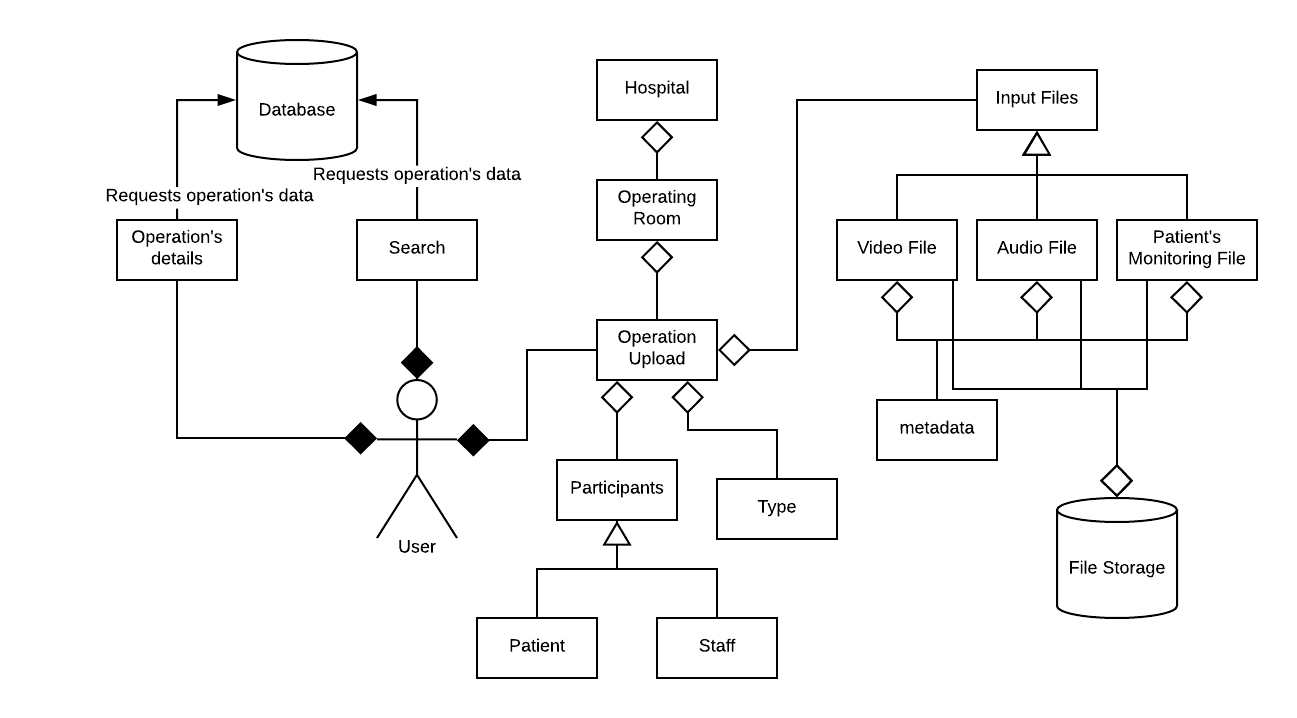
\includegraphics[width=17cm]{imgs/Domain_Model.png}
\end{center}\vspace{-0.3cm}
\caption[Domain Model]{Conceptual model of the system's problem domain} \label{domain_model}
\end{figure}



\section{Use Case Analysis}
\label{sub:use_case_analysis}

Following the domain modelling and the gathering of requirements analysed in sections \ref{sec:DomainModelling} and \ref{sec:softreqlistandprior} respectively, use cases were developed. The defined domain entities and requirements were used to construct the use cases and their basic relationships. The construction of the uses cases allows the solid organisation of the functional requirements of the project, in order to make sure that they meet the front-end requirements and also to make sure that they are fully encompassing. A use case describes a scenario where a user interacts with the application in order to achieve a specific outcome \cite{usecases3}. Use cases are described from the users point of view rather than a technical point of view. As such, use cases are very effective at visualising and communicating the final product to the client and incorporating the client's voice into the requirements of the project \cite{usecases2}.

A complete overview of the identified use cases is shown in  Table \ref{UC-Summary} and from Table \ref{UC01} to Table \ref{UC03}, all the detailed specification for each use case are shown. Each specification includes details of each use case,the main flows, error flows, post-conditions, pre-conditions and the trigger event.


\begin{table}[h]
\centering
\begin{tabular}{|
>{\columncolor[HTML]{C0C0C0}}p{1.5cm}|p{8cm}|}
\hline
\textbf{ID} & \cellcolor[HTML]{C0C0C0}\textbf{Use Case}  \\ \hline
UC01        & \textbf{Upload a new operation}                           \\ \hline
UC02        & \textbf{Search for an operation}                             \\ \hline
UC03        & \textbf{View operation detals}                                                         \\ \hline
\end{tabular}
\caption[Use Case Listing]{List of use cases}
\label{UC-Summary}
\end{table}


\begin{table}[h]
\footnotesize
\centering
\begin{tabular}{|
>{\columncolor[HTML]{C0C0C0}}p{2.7cm}|p{12cm}|}
\hline
Use Case          & Upload a new operation \\ \hline
ID                & UC01                                                                                                                                                                                                                                                                                          \\ \hline
Brief Description & The user wishes to register the operation to the System                                                                                                                                                                                                                         \\ \hline
Preconditions     & User must have all the necessary files and information of the operation                                                                                                                                                                                                                                         \\ \hline
Main Flow         & \begin{tabular}[c]{@{}l@{}}1. Home page is displayed\\ 2. The User selects to register a new operation\\ 3. The User enters the hospital name \\ 4. The User enters the operating room number \\ 5. The User enters all the staff that participated in the operation\\6. The User enters the patient that underwent the surgery\\ 7. The User enters the type of the operation\\ 8. The User selects all the relevant video files \\9. The User selects all the relevant audio files \\10. The User selects the patient's monitoring file \end{tabular}                                                                      \\ \hline
Post Conditions   & A new operation has been registered to the database and the files have been uploaded to the file storage                                                                                                                                                                                                                                                        \\ \hline
Alternative Flows & The User no longer wishes to upload yet the operation to the System and cancels the registration of the operation                                                                                                                                                                                                        \\ \hline
Error Flow        & \begin{tabular}[c]{@{}l@{}}1. The User does not enter any of the 1-7 fields and at least one input file \\ 2. An error message is displayed \end{tabular} \\ \hline
Trigger Event     & The user chooses to add new operation \\ \hline
\end{tabular}
\caption[Use Case 01 - Upload a new operation]{Use Case 01 - Upload a new operation}
\label{UC01}
\end{table}


\begin{table}[h]
\footnotesize
\centering
\begin{tabular}{|
>{\columncolor[HTML]{C0C0C0}}p{2.7cm}|p{12cm}|}
\hline
Use Case          & Search for an operation \\ \hline
ID                & UC02                                                                                                                                                                                                                                                                                          \\ \hline
Brief Description & The User wishes to find an operation from the database \\ \hline
Preconditions     & At least one operation must have been registered to the system \\ \hline
Main Flow         & \begin{tabular}[c]{@{}l@{}}1. Home page is displayed\\ 2. The 20 most recent uploaded operations are displayed\\ 3. The User uses the Filters to input hospital name,operating room number,\\ from/to date and participated staff  \\ 4. The filtered results are displayed, ordered by date (from most recent to oldest) \end{tabular}                                                                      \\ \hline
Post Conditions   & The User can see the Operations that correspond to the Filters they have applied \\ \hline
Alternative Flows & The Operation that the User searches for and the Filters applied produce no results \\ \hline
Error Flow        &  None \\ \hline
Trigger Event     & The User wishes to Search for an Operation \\ \hline
\end{tabular}
\caption[Use Case 02 - Search for an operation]{Use Case 02 - Search for an operation}
\label{UC02}
\end{table}


\begin{table}[h]
\footnotesize
\centering
\begin{tabular}{|
>{\columncolor[HTML]{C0C0C0}}p{2.7cm}|p{12cm}|}
\hline
Use Case          & View operation details \\ \hline
ID                & UC03 \\ \hline
Brief Description & The User can view the details of an Operation \\ \hline
Preconditions    & \begin{tabular}[c]{@{}l@{}}1. At least one operation must have been registered\\ 2. The User must have searched for an Operation\\  \end{tabular}                                                                      \\ \hline
Main Flow         & \begin{tabular}[c]{@{}l@{}}1. Home page is displayed\\ 2. The User searches for an Operation\\ 3. The User views the filtered results  \\ 4. The User selects the desired Operation \\ 5.The User views the Operation details \end{tabular}                                                                      \\ \hline
Post Conditions   & The Operation details are displayed to the User \\ \hline
Alternative Flows & The User does not wish to view the Operation details and so goes back to the homepage \\ \hline
Error Flow        &  System fails to report Operation Details \\ \hline
Trigger Event     & The User wishes to view the details of a listed Operation \\ \hline
\end{tabular}
\caption[Use Case 03 - View operation details]{Use Case 03 - View operation details}
\label{UC03}
\end{table}


\section{Use Case Diagram}
\label{sub:use_case_diagram}


The use case diagram which is depicted in Figure \ref{UC-diagram} is derived from the use case Listing which is basic foundation for the creation of the use case diagram.


\begin{figure}[h]
\begin{center}
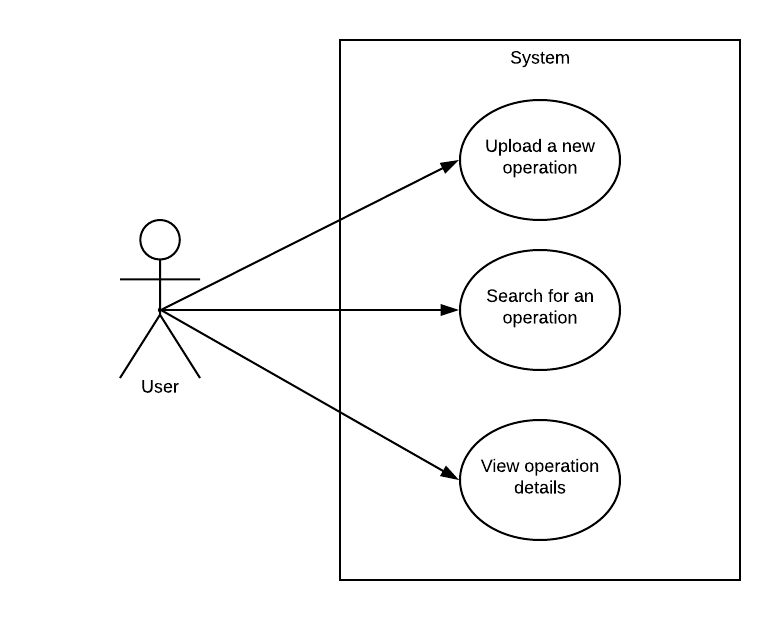
\includegraphics[width=17cm]{imgs/Use_Case_Diagram.png}
\end{center}\vspace{-0.3cm}
\caption[Use Case Diagram]{Use case diagram} \label{UC-diagram}
\end{figure}

\section{List of Views}
\label{sub:List_Of_Views}

The Use Cases identify 3 main views that were needed in the project. The first one is the ``Add new Operation" View where the user can register a new operation to the system. 


one is the ``Search for an Operation'' view which is also the Home Page. This is the first screen that the user sees and it is used to display the 20 most recent uploaded operations. The user can also apply specific filters like hospital, operating room number, specific patient etc., in order to limit the result and find a specific operation of interest. 





\chapter{Design and Implementation}
\label{chapterlabel4}

The analysis performed in Chapter \ref{chapterlabel3} allows a full outline of the system requirements, the entities of the system and their assigned interactions, and leads onto the development of the full design of the software. The design phase starts with the design and the architecture of the system that is going to be built.




\section{Architecture and System Structure}
\label{Architecture_And_System_Structure}

The system is a typical B/S (Browser/Server) framework with a client browser sending requests and responses and a Kestrel server which is the default cross-platform HTTP server for ASP.NET Core projects. The server is running c\# (version 7.0) with a MySQL database. The server implementation listens for HTTP requests and surfaces them to the app as sets of request features composed into an HttpContext \cite{aspNetStructure}. ASP.NET Core communicates with the MySQL database which is hosted in Azure. The structure of ASP.NET Core is shown in figure \ref{asp_structure}.



\begin{figure}[h]
\begin{center}
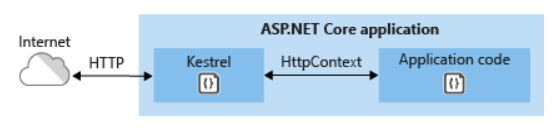
\includegraphics[width=17cm]{imgs/asp_structure.jpg}
\end{center}\vspace{-0.3cm}
\caption[ASP.NET Structure]{ASP.NET Structure} \label{asp_structure}
\end{figure}


The architectural framework is divided into four basic tiers: front-end, back-end, database, and file storage.

\begin{enumerate}
\item \textbf{Front-End}: the front end is user interface where the user completes a series of operations to control the application which is supported by HTTP request and HTTP response. It contains HTML code, JavaScript, JQuery and CSS)

\item \textbf{Back-End} when a static HTTP response is received from the web browser, ASP.NET Core will create an HttpRequest object that contains the request data, and invoke the correspondent view to handle this object. After the handle process, it will create and return a new HttpResponse object to the front-end view.
\item \textbf{Database}: ASP.NET Core controls the MySQL relational database which is hosted in Azure.
\item \textbf{File Storage}: The files selected by the user are uploaded to Azure Blob Storage.


\end{enumerate}

\begin{figure}[h]
\begin{center}
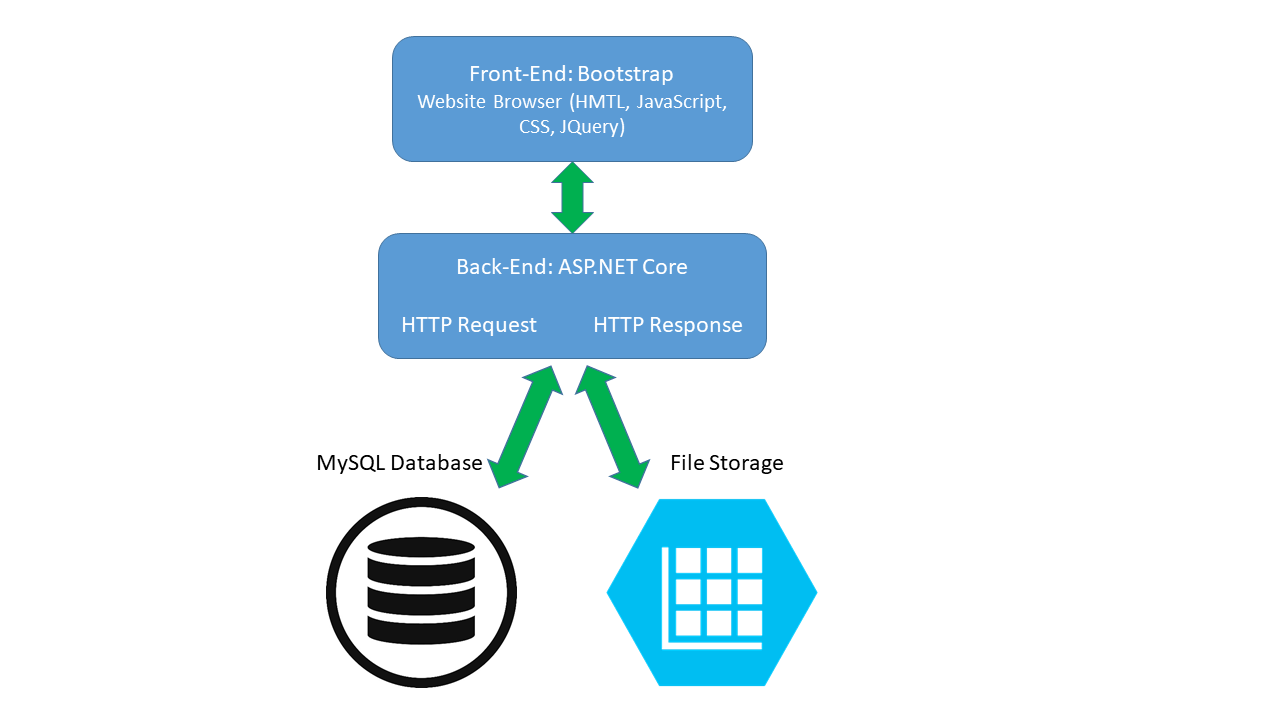
\includegraphics[width=17cm]{imgs/Application_Structure.png}
\end{center}\vspace{-0.3cm}
\caption[Application General Structure]{Application General Structure} \label{app_Structure}
\end{figure}


\section{Model-View-Controller Pattern}
\label{sub:MVC}

Due to the time limitations of the project the lack of experience in web designing, it was more appropriate to create a basic user interface and the devote the majority of the time to developing a robust back-end. Therefore, it was very important that the architecture of the application made a separation between the user interface and the back-end processing.

MVC framework is a one of the most popular design patterns which is motivated by the separation of the  UI and the processing performed to generate it. The MVC has been conceptualised for many years, and thus it precedes the inception of web applications and therefore, many efforts at applying the model to web applications through frameworks have been controversial.

Since most of the time has been devoted into developing the back-end than the front-end of the application, it is quite likely that at some point in the future the front-end would be replaced with a more aesthetically pleasing one.


The Model-View-Controller (MVC) architectural pattern separates an application into three main groups of components: Models, Views, and Controllers. This pattern helps to achieve separation of concerns \cite{separationOfConcerns}. Using this pattern, user requests are routed to a Controller which is responsible for working with the Model to perform user actions and/or retrieve results of queries. The Controller chooses the View to display to the user, and provides it with any Model data it requires \cite{mvc}. 

\begin{figure}[h]
\begin{center}
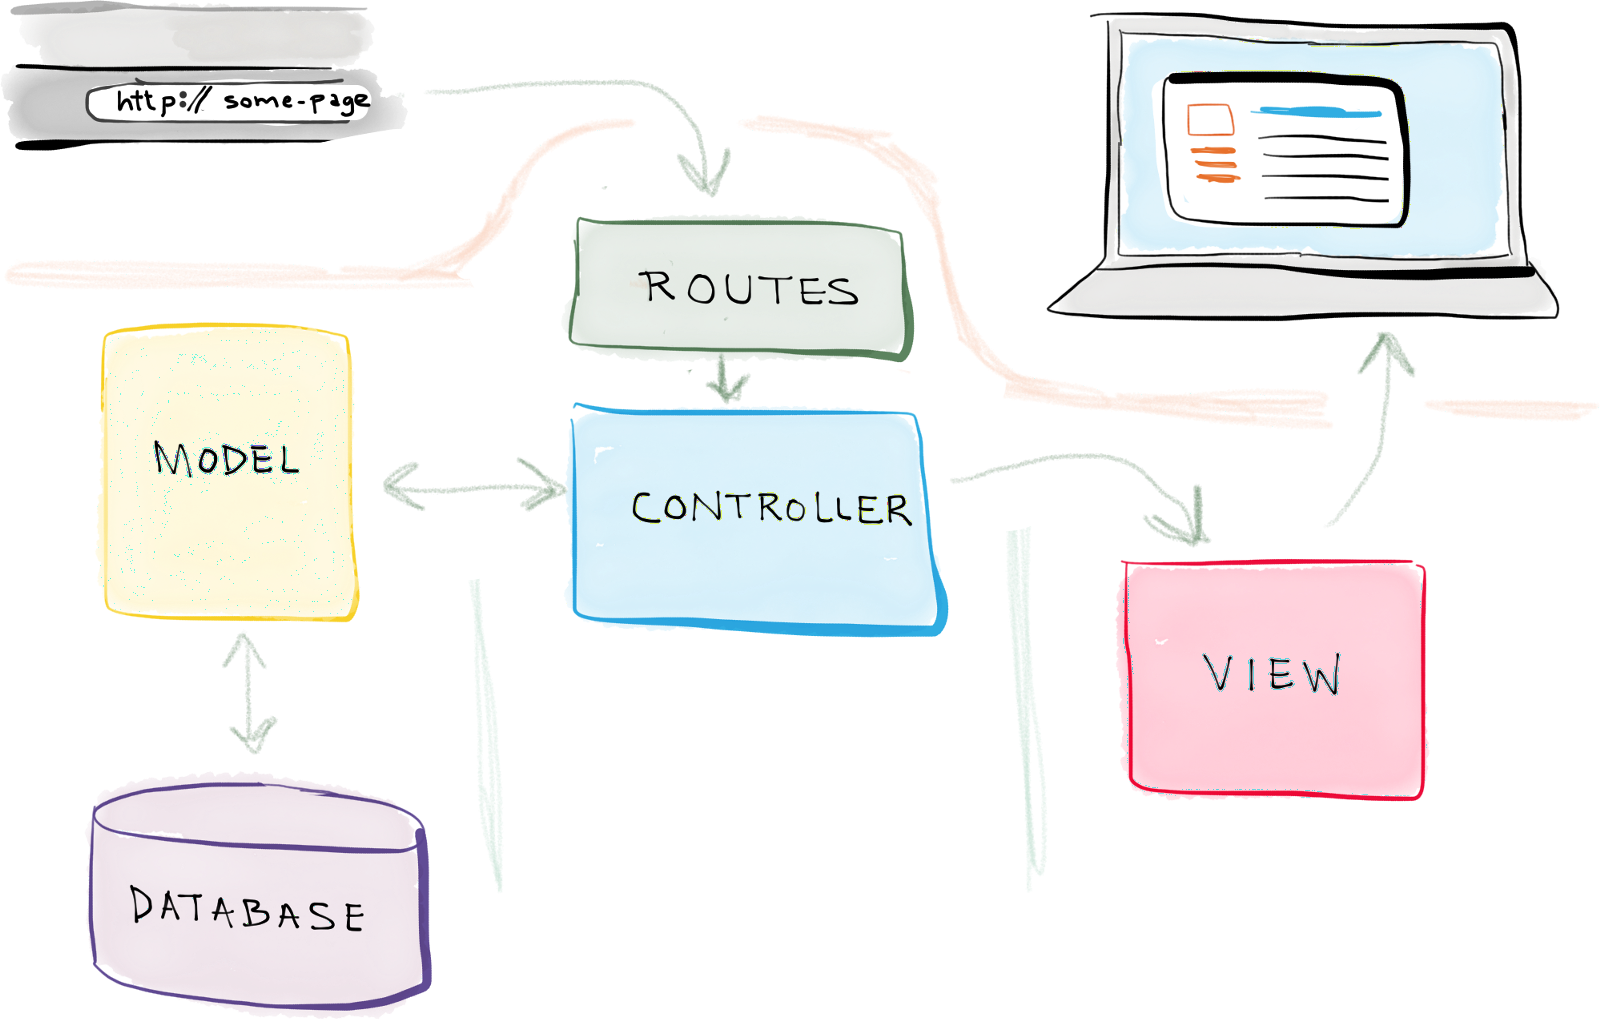
\includegraphics[width=17cm]{imgs/mvc.png}
\end{center}\vspace{-0.3cm}
\caption[The Model-View-Controller Pattern of ASP.NET Core]{The Model-View-Controller Pattern of ASP.NET Core} \label{mvc}
\end{figure}


The server-side MVC (Model-View-Controller) framework (as depicted in figure \ref{mvc} has three core layers:

\begin{enumerate}
\item \textbf{The Model}: The Model in an MVC application represents the state of the application and any business logic or operations that should be performed by it.\cite{mvc}. This is essentially a library of supporting methods which help the Controller in generating the data to pass to the View. Those methods are especially written to handle  and populate data related to the particular View and are based on libraries of more generic functions built to provide helping functions to the Model tier.

\item \textbf{The View} Views are responsible for presenting content through the user interface. In ASP.NET Core Views use the Razor view engine which is a compact, expressive and fluid template mark-up language for defining views using embedded C\# code.  Razor is predominantly used to dynamically generate web content on the server and allows to cleanly mix server code with client side content and code. \cite{mvc}. Razor view engine is also used for the opposite; embed c\# code in HTML mark-up. As a general principle, there should be minimal, if not none, logic within the views, and any logic should be related to presenting the content/model, passed from the Controller.

\item \textbf{The Controller}: This is a set of classes that manages the relationship between the View and the Model\cite{mvcBook}. It responds to user input, communicates with the Model, and ``decided'' which view to render and send back to the client side. Essentially, it controls the application logic for a particular unit and is responsible to call all the necessary methods from the Models in order to generate and pass the correct data to the View.

\end{enumerate}

\section{Design Class Diagram}
\label{design_class_diagram}


The design class diagram represents a complete overview of the classes within the system, the methods they use and the links between them. On of the main aims of designing the class diagram, is to achieve high cohesion and low coupling. The design class diagram, shown in Figure \ref{DesignClassDiagram} fully details all the internal entities of the system and maps the structure of the components of the software. As explained in subsection \ref{sub:MVC} the controller classes contain methods which are responsible for handling all entities of the system and updating specific states during their life-cycles, depending on the performed action. The notation used for this diagram is based on common industry notation for class diagrams \cite{entity_relationship_approach} \cite{object_oriented_modeling_and_design}.


\clearpage

\begin{landscape}
\begin{figure}[h]
\begin{center}
\thispagestyle{empty}
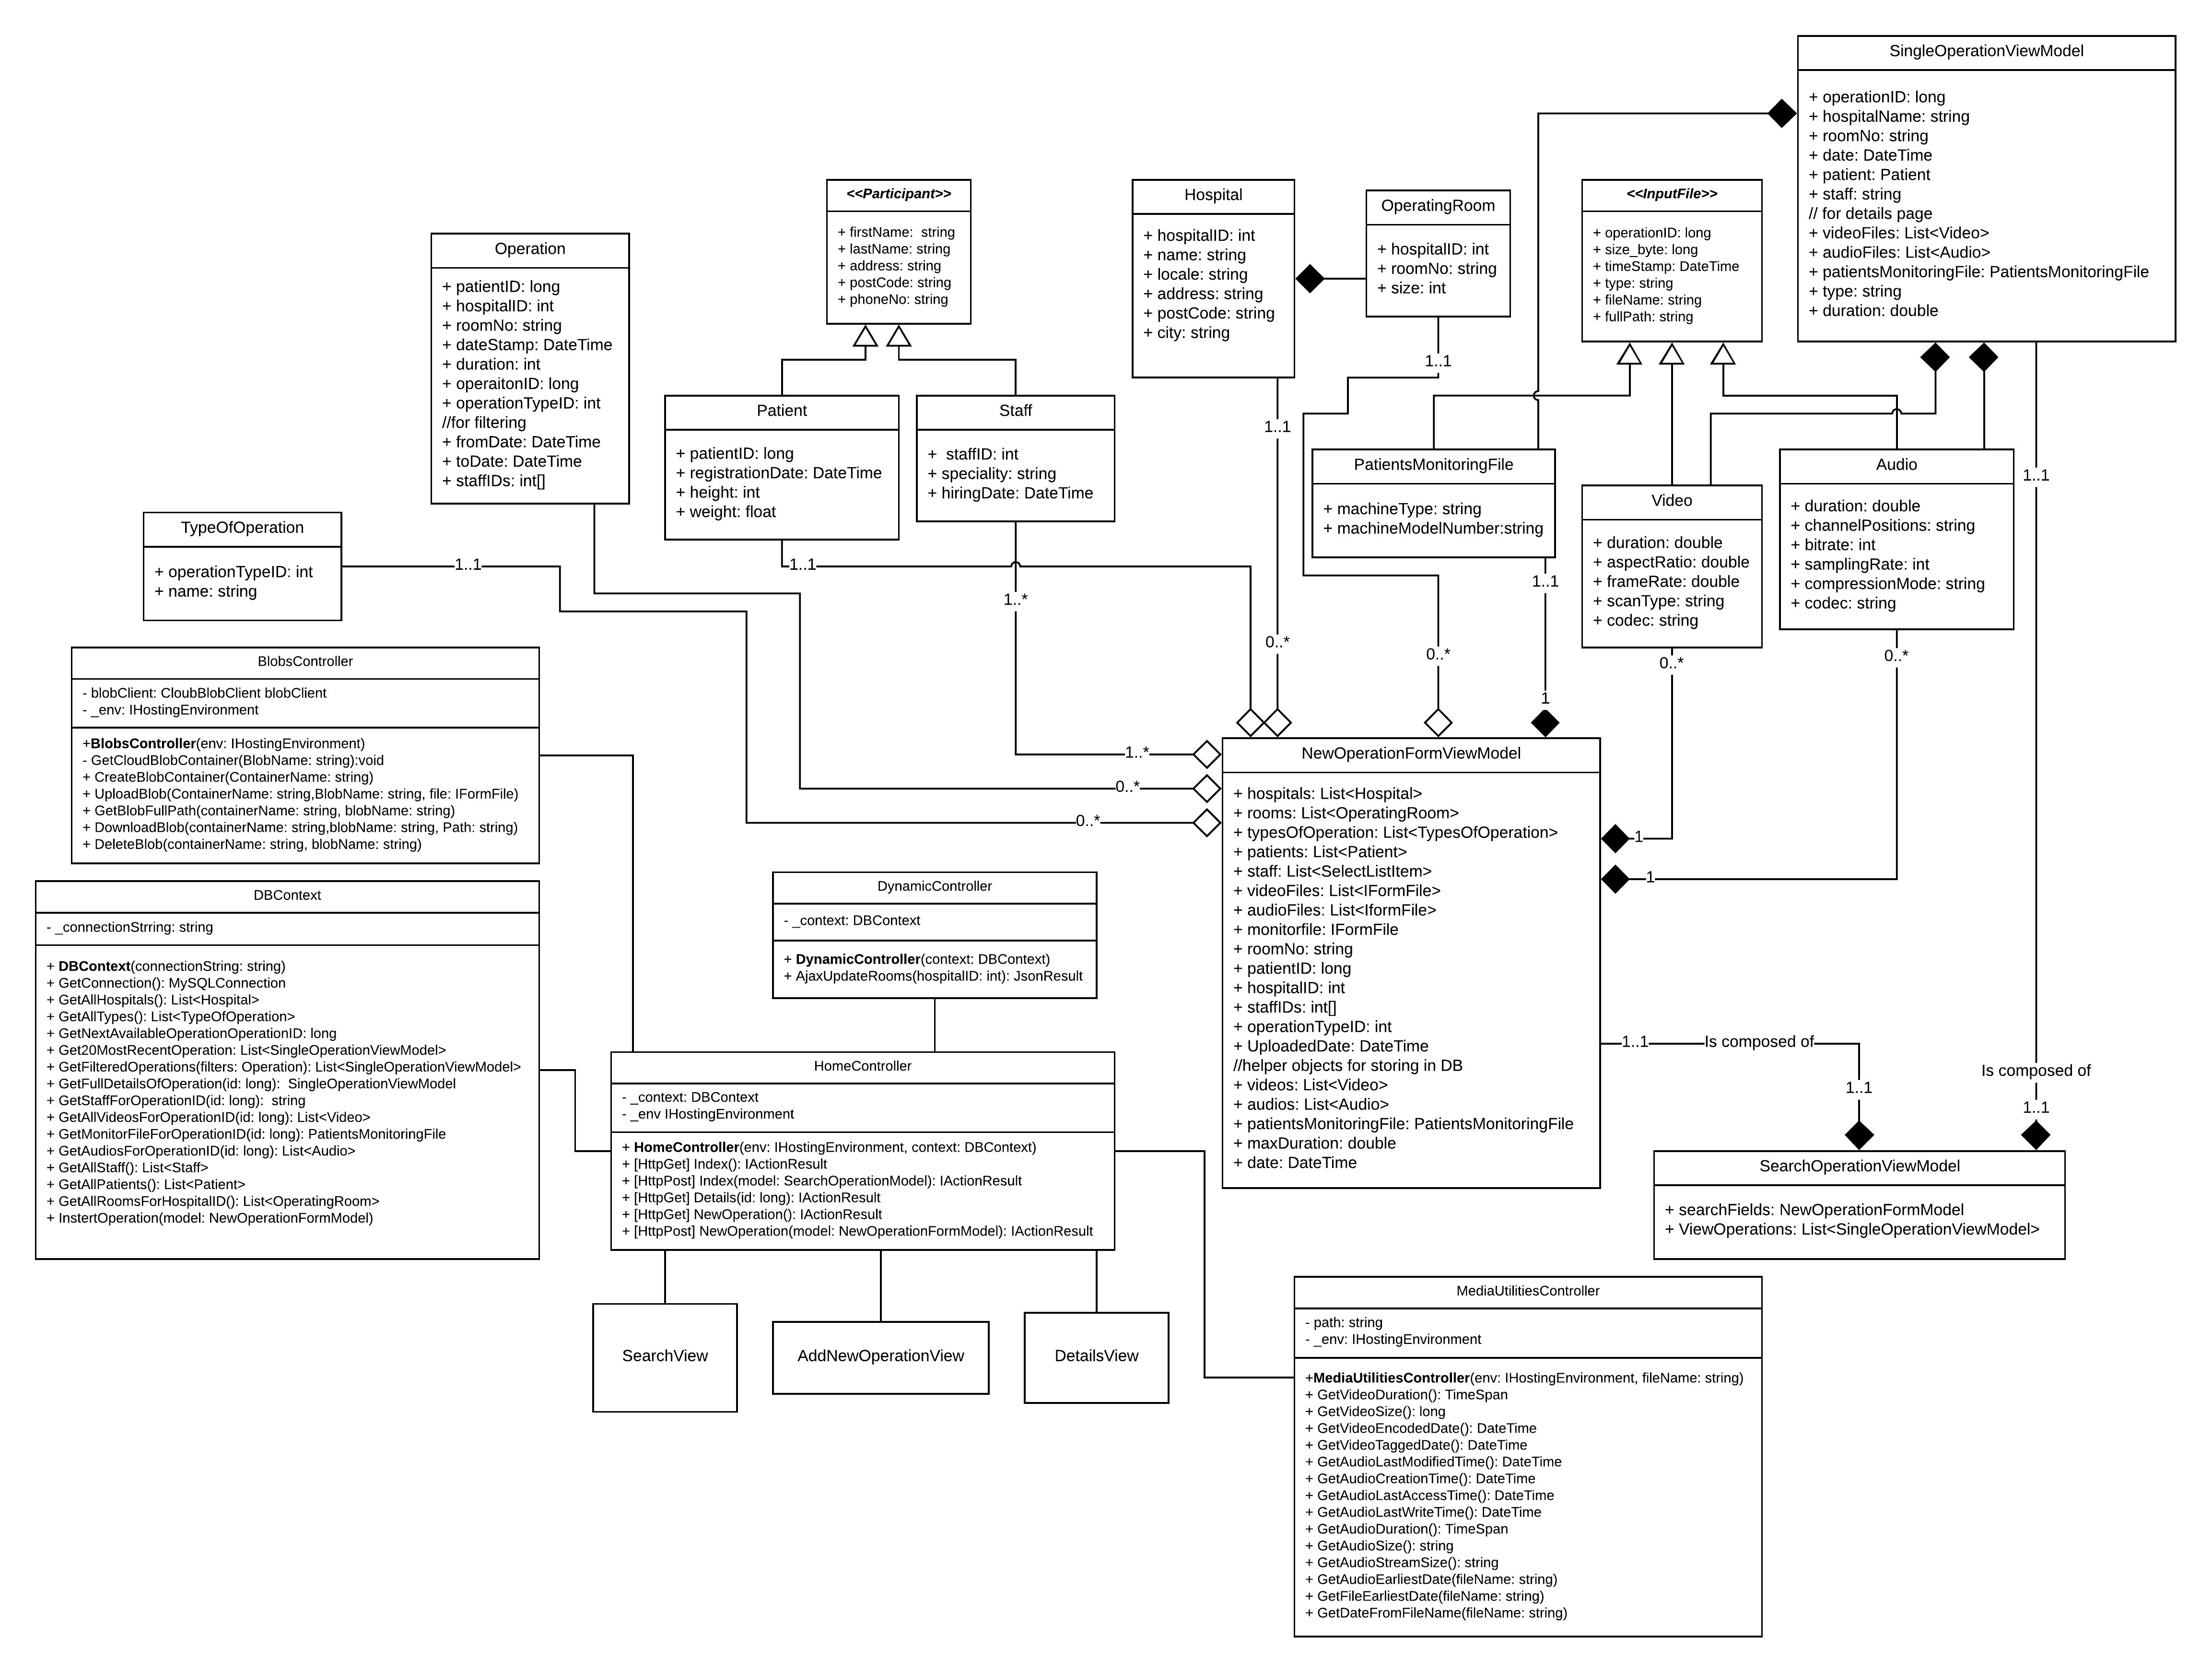
\includegraphics[width=24cm]{imgs/Design_Diagram.png}
\end{center}\vspace{-0.3cm}
\caption[Design Class Diagram]{Design class diagram.} \label{DesignClassDiagram}
\end{figure}
\end{landscape}
\newpage

 
\section{Database Design}
\label{database_design}

\subsection{Introduction}
\label{sub:intro}
A database is a data repository where the data is managed and stored according to the data structure.  It enables data sharing across an organisation, reduces data redundancy and increases data consistency. Database development doesn't have a unique way of implementing, and different data structures require different types of database. In regards to this application, the relational database was selected to represent the data structure. The main purpose of relational databases is to examine how data is related to each other. They translate the complicated data structure and data relationship into simple two-dimensional tables. In the relational model, data and relationships are represented as tables, each of which has a number of columns with a unique name.

Regarding this specific application, it was deemed that a MySQL\cite{mysql} database is the most suitable relational database management system. MySQL is an easy to use, reliable, scalable and specifically designed and optimized for Web Applications. Although it requires additional configuration when the application is deployed in the server, it is powerful enough to support the extensive complexity that the current application needs.

\subsection{Conceptual Schema}
Conceptual modeling or conceptual database design is the process of constructing a model of the information use in an enterprise that is independent of implementation details, such as the target DBMS, application programs, programming
languages, or any other physical considerations. This model is called a conceptual
data model\cite{Database_Systems}. The Conceptual Schema is shown in figure \ref{conceptual_schema}.


\begin{figure}[h]
\begin{center}
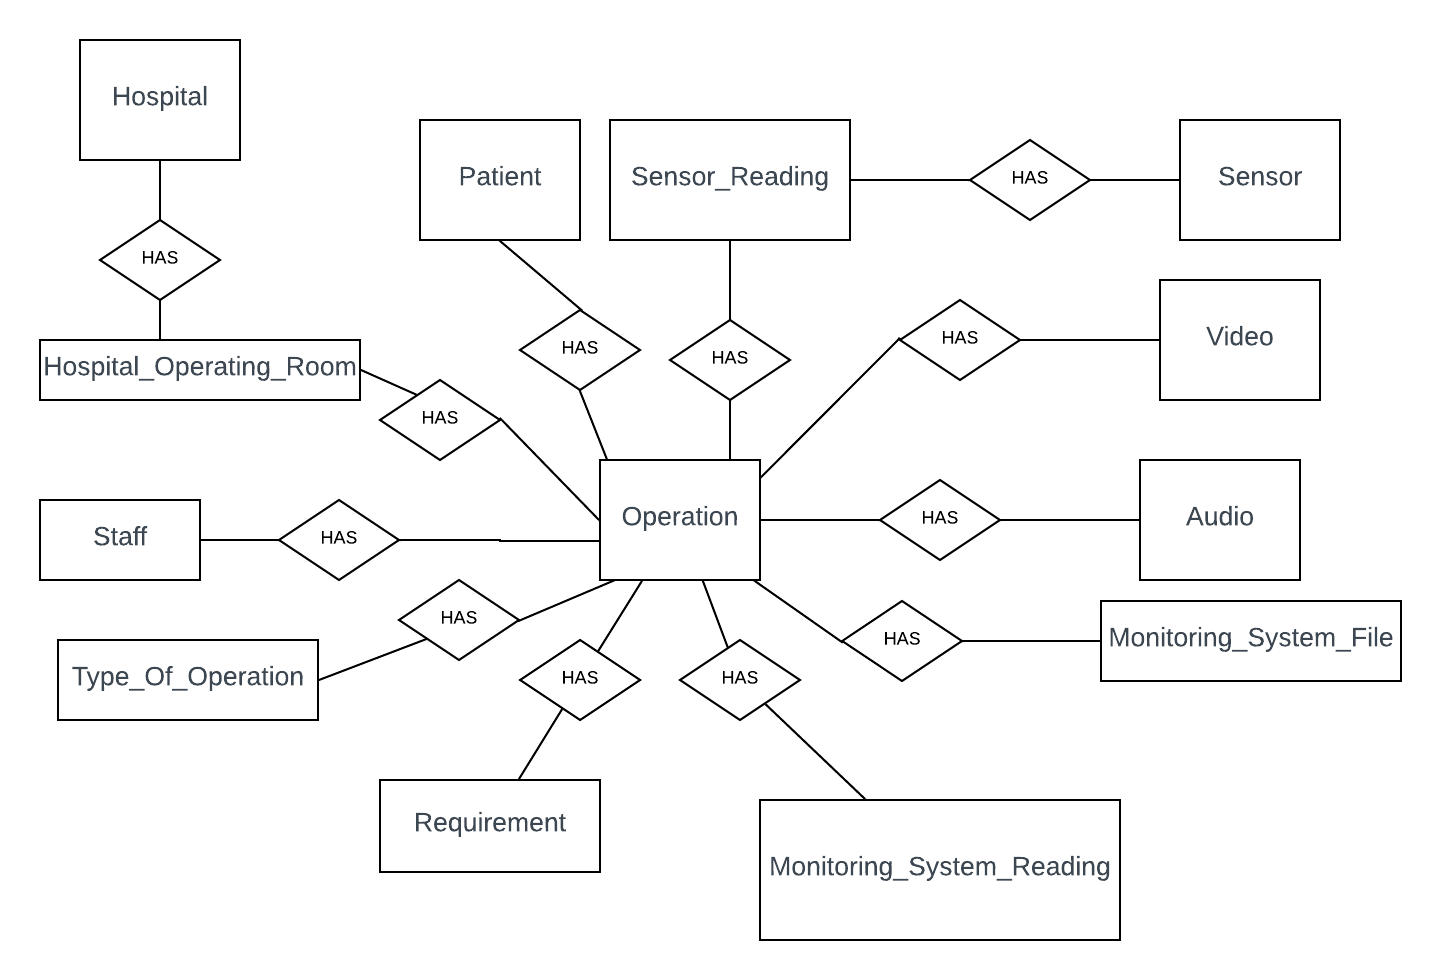
\includegraphics[width=17cm]{imgs/conceptual_schema.png}
\end{center}\vspace{-0.3cm}
\caption[Conceptual schema]{Conceptual schema} \label{conceptual_schema}
\end{figure}



\subsection{Logical Schema}

The logical database design phase maps the conceptual data model on to a logical model, which is influenced by the data model for the target database. The logical data model is a source of information for the physical design phase, providing the physical database designer with a vehicle for making trade-offs that are very important to the design of an efficient database \cite{Database_Systems}

While the conceptual model is independent of all implementation details, the logical model assumes knowledge of the underlying data model
of the target DBMS. The Entity Relationship diagram (Figure \ref{er_diagram}) is created based on the analysis of logical schema. All attributes of every entity have been labelled in the diagram.


\begin{figure}[h]
\begin{center}
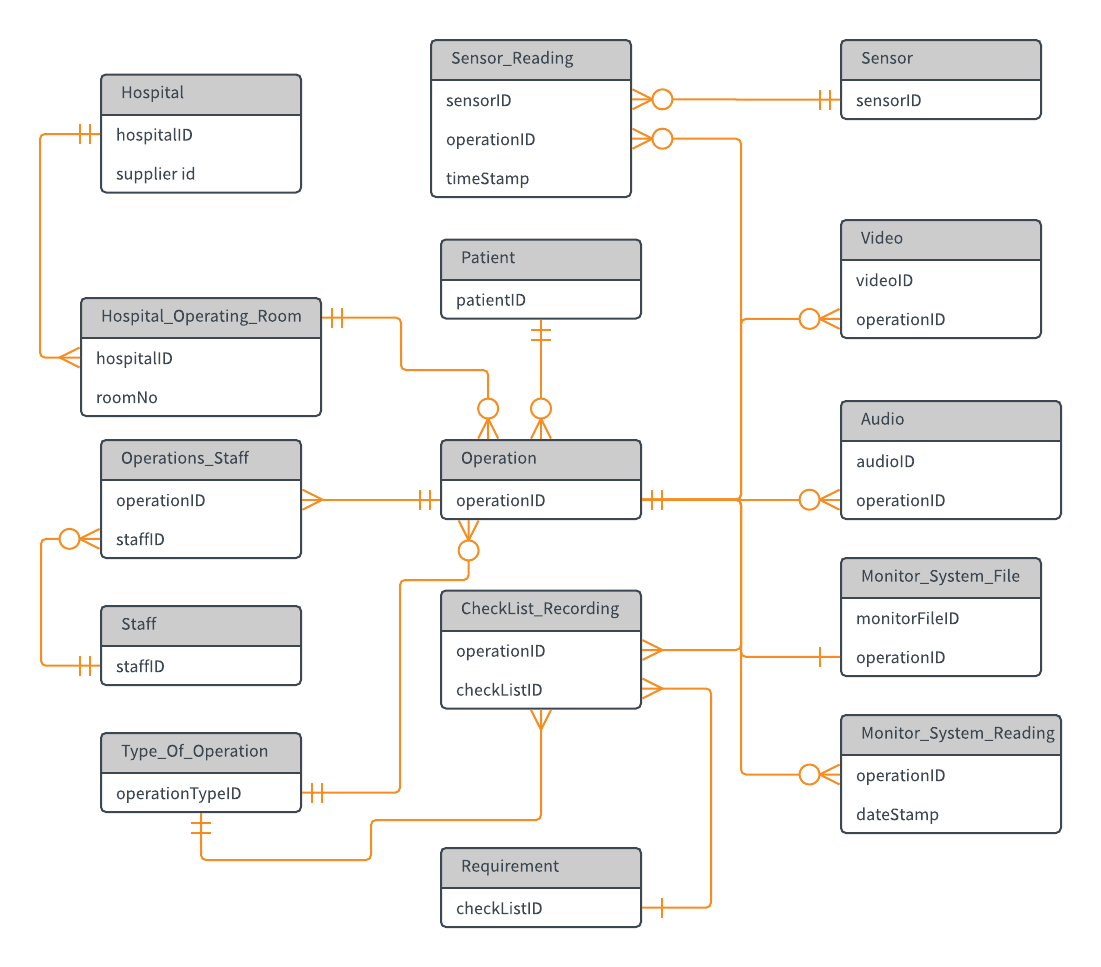
\includegraphics[width=17cm]{imgs/er_diagram.png}
\end{center}\vspace{-0.3cm}
\caption[Entity-Relationship Diagram]{Entity-Relationship Diagram} \label{er_diagram}
\end{figure}


\subsection{Physical schema}

In this final phase of the database design methodology, the logical database design (entities, attributes, relationships, and contrains) has to be translated into a physical database design that can will be implemented using the target DBMS, which in this case in a MySQL database hosted in Azure. Each attribute in the physical schema ( Figure  \ref{physical_schema} ) has constrains which prevent storing invalid data and quickens up the data validation process, requiring no additional code to rewrite the data validation interfaces. The physical database has been especially designed in order to require minimal work for new sensor adding. For example, if a new sensor is added in the future, the  schema wouldn't have to be changed and a single row in the ``Sensor'' table is the only required action. Each sensor reading is recorded to the ``Sensor\_Reading'' relation.

\begin{figure}[!ht]
\begin{center}
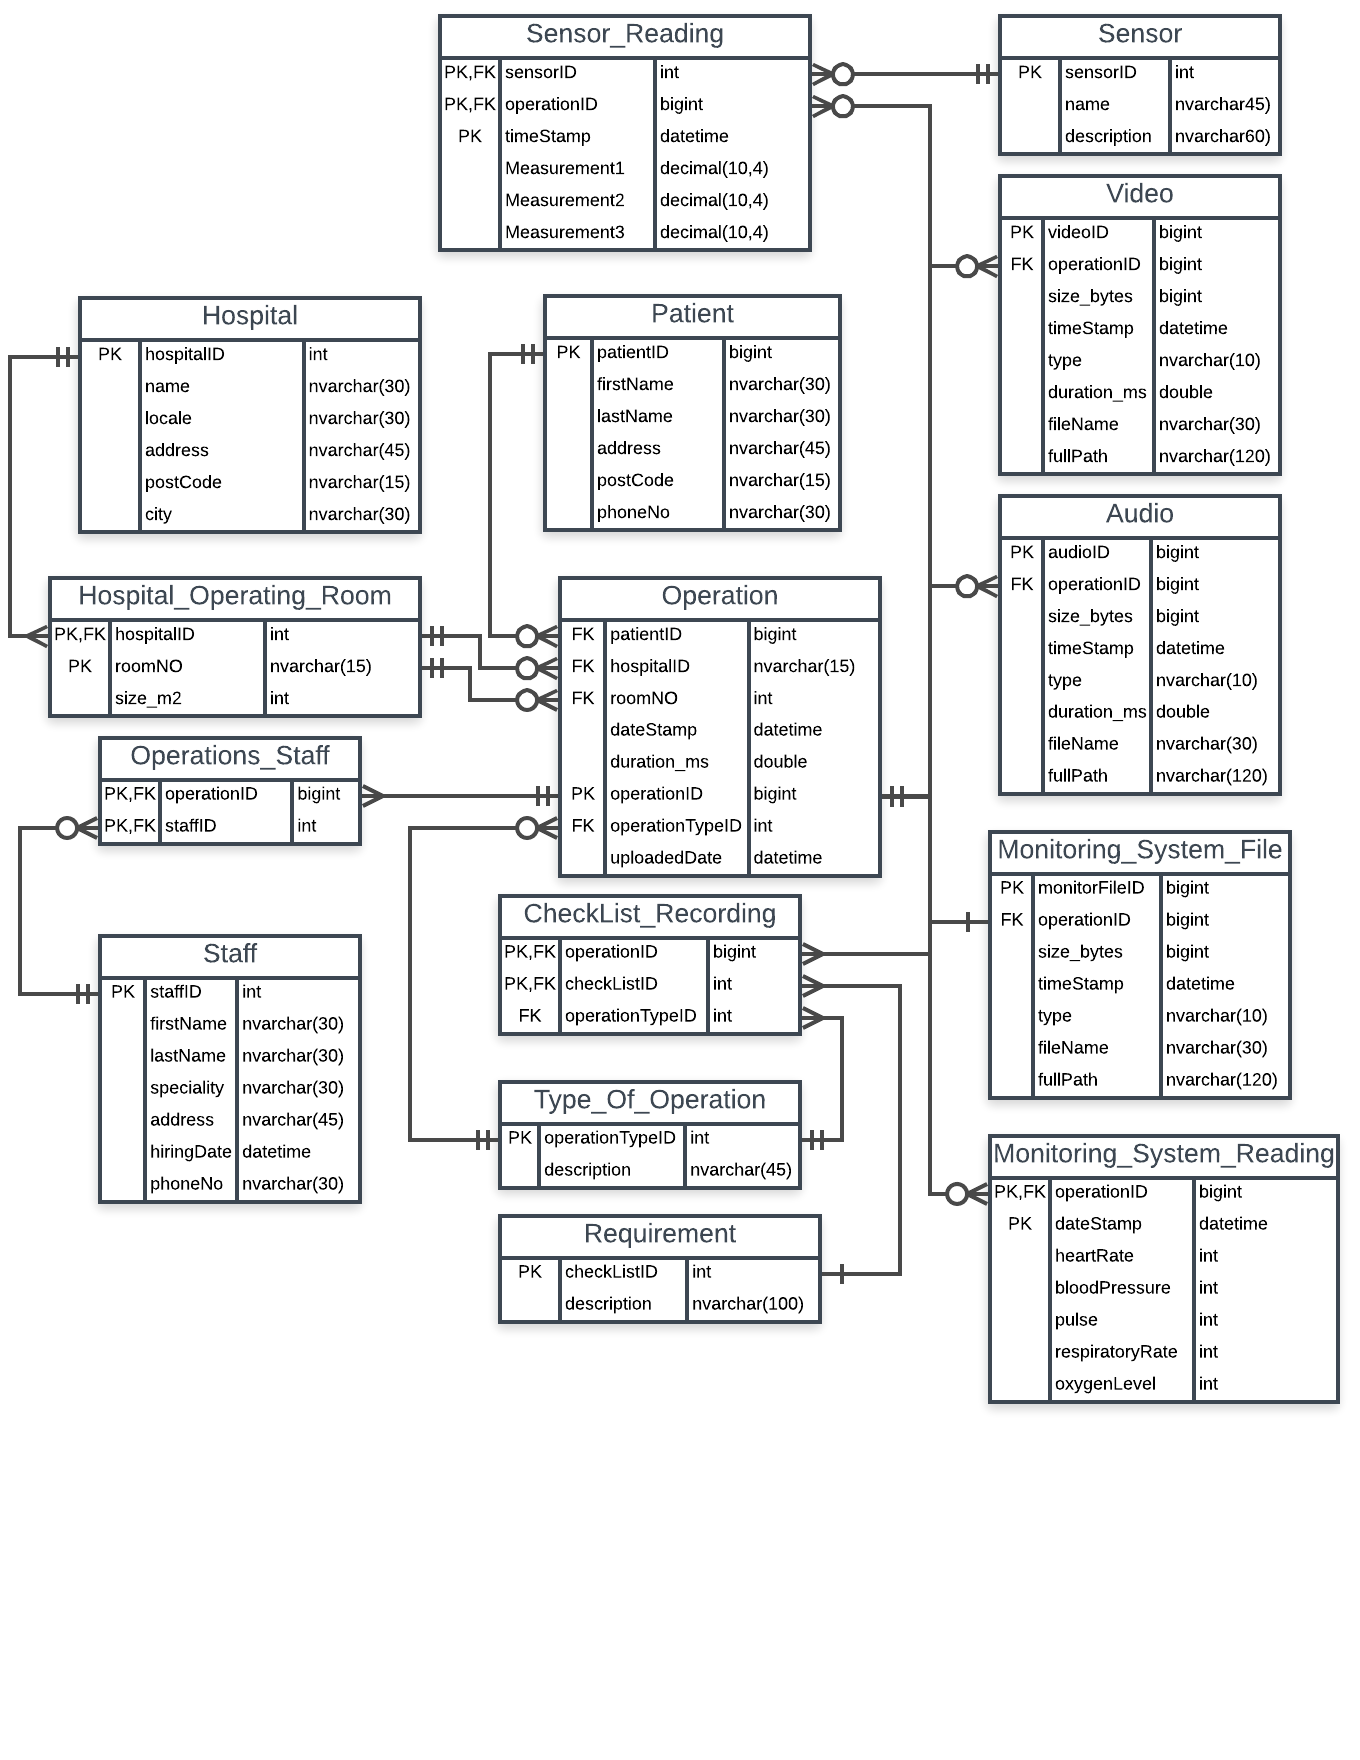
\includegraphics[width=17cm]{imgs/physical_schema.png}
\end{center}\vspace{-0.3cm}
\caption[Physical database schema]{Physical database schema} \label{physical_schema}
\end{figure}

\section{Pages Implementation}
\label{sec:pages_implementation}

Since, the front-end part of the application is fairly straight-forward, the implementation stage will be split into three subsection which are also the three main views of the application. The first part of the implementation is the page where the user can upload a new operation, the second part is where the user can make a search for a specific operation stored in the relational database and choose an operation of their choice, and the third page is where the user can see all the details that are related to the specific operation.
The application has a single Controller, which as mentioned in \ref{sub:MVC}, is an interface between the Model and the View components, processes all the logic and incoming requests, manipulates data using the Model component and interacts with the Views to render the final output. In the HomeController of the application, there are three main methods that correspond to the three main views, which will be analysed in detail in the following subsections. 


\subsection{``Register new operation'' Implementation}
\label{sub:register_new_operation_implementation}

In this subsection, the process of registering a new operation to the system is explained. The HomeController of the application has two methods with exactly the same names (``New Operation'') that correspond to the HttpGet and HttpPost request from the client side. When the user selects to load the ``Add new Operation'' View, the HttpGet method is called from the Controller. Due to the fact that this page doesn't require a already defined model of the application, a new ViewModel had to be created (``NewOperationViewModel''). 
At this stage, the controller instantiates the ViewModel, queries the database to load it and then passes it to the rendered View for display. The HttpGet method of the HomeController is shown in figure \ref{new_operation_get}.


\begin{figure}[!ht]
\begin{center}
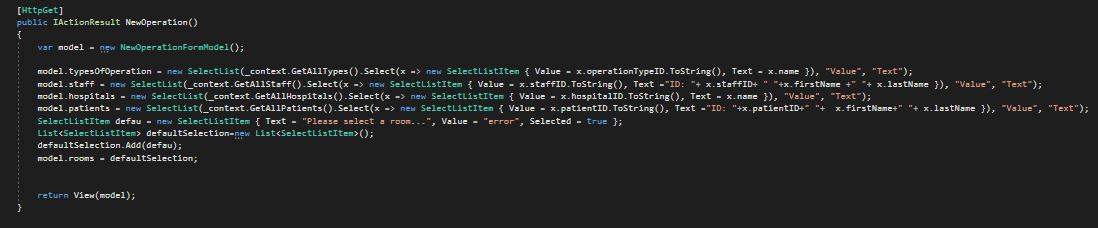
\includegraphics[width=17cm]{imgs/new_operation_get.jpg}
\end{center}\vspace{-0.3cm}
\caption[NewOperation (HttpGet Request)]{NewOperation (HttpGet Request)} \label{new_operation_get}
\end{figure}

After the model is passed to the view, all the information, in regards to the model, will be displayed. The user here, enters all the information related to the specific operation (hospital, operating room, participated staff) and uploads the input files that have been extracted from the sensors. The information entered from the user are passed to the server using the ASP.NET Core MVC Model Binding. Model binding in ASP.NET Core MVC maps data from HTTP requests to action method parameters. When MVC receives an HTTP request, it routes it to a specific action method of a controller. It determines which action method to run based on what is in the route data, then it binds values from the HTTP request to that action method's parameters \cite{modelBinding}.

Before the web application posts back to the server, JavaScript validation has to be performed to ensure that the user conforms with the application's requirements. More specifically, the user has to select a value from all the dropdown menus, and select at least one video file or one audio file or the patient's monitoring system file. The user interface that the user uploads a new operation is shown in figure \ref{new_operation_page}. It is important here to mention that the field ``Operating Room'' depends on the selection of the specific hospital and cannot be pre-populated. Therefore, a request had to be submitted to the server without posting back and so AJAX had to be used. The section where the client sends a request to the server, in order to query the database and return a JSON object is shown in figure \ref{ajax}


\begin{figure}[!ht]
\begin{center}
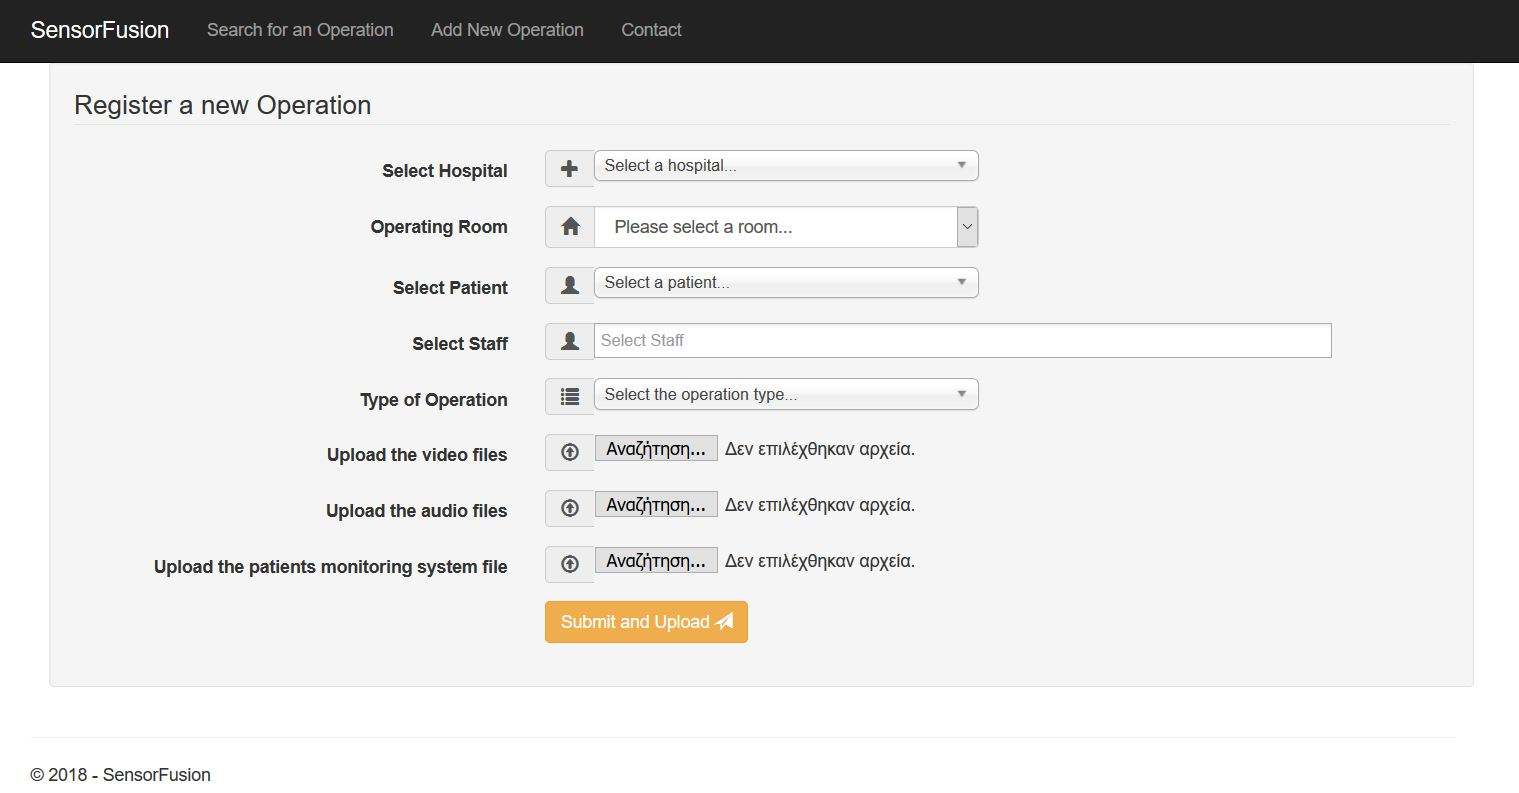
\includegraphics[width=17cm]{imgs/new_operation_page.jpg}
\end{center}\vspace{-0.3cm}
\caption[NewOperation Page]{NewOperation Page} \label{new_operation_page}
\end{figure}

\begin{figure}[!ht]
\begin{center}
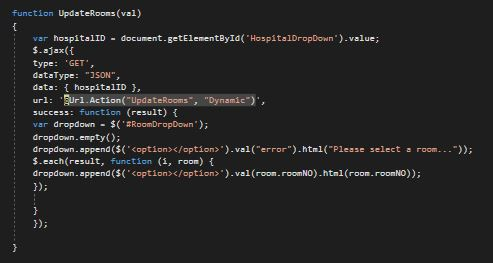
\includegraphics[width=17cm]{imgs/ajax.jpg}
\end{center}\vspace{-0.3cm}
\caption[AJAX Call]{AJAX Call} \label{ajax}
\end{figure}

When the user has entered all the required fields and selected at least one input file for uploading, a HttpPost request is submitted to the server. As previously mentioned, model binding in ASP.NET Core easily binds the data coming from the View to the model, which is then passed back to the controller for manipulation. When the user submits the form, another method with the same name is called (``NewOperation'') which is responsible for the HttpPost requests and takes as input the ViewModel (NewOperationFormViewModel).
After the server-side validation of the model has been successful, the controller must process and manipulate the incoming data, store the input files in the Azure blob storage and insert the new operation to the MySQL relational database. For the purpose of communicating with the database, an additional class has been created (DBContext). The controller, takes as input the model originated from the View, manipulates the incoming data, and passes the same model to the ``DBContext'' class for updating the database. This is a very important issue, as the application had to follow the principle of separation of concerns.
It is very critical here to mention that only the metadata extracted from the input files were stored to the MySQL database. The files themselves were only stored to a connected file storage account (Microsoft Azure Blob Storage). For this purpose, a new controller had to be created in order to store and retrieve the files from the file storage (BlobsController).

In regards to the extraction of the meta-data from the input files, additional NuGet packages and libraries (MediaInfo) had to be installed to the project. Furthermore, a dedicated class for processing, manipulating and extracting metadata from the files had to be created (``MediaUtilities''). This class enables the application to extract information from the input files that would have otherwise been almost impossible to gain. A very small sample of the obtained metadata include the exact starting date, the size of the files, codec used, encoded date, aspect ratio, frame-rate, duration of the media files and many more. The part where the application extracts the metadata from the media files is shown in figures \


\begin{figure}[!ht]
\begin{center}
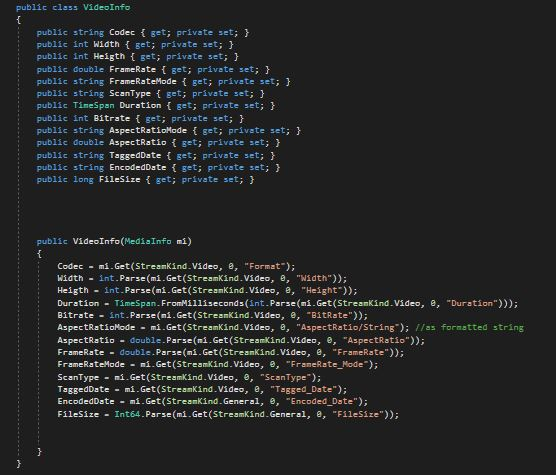
\includegraphics[width=17cm]{imgs/video_extracting.jpg}
\end{center}\vspace{-0.3cm}
\caption[Extracting meta-data from video files]{Extracting meta-data from video files} \label{video_extracting}
\end{figure}

\begin{figure}[!ht]
\begin{center}
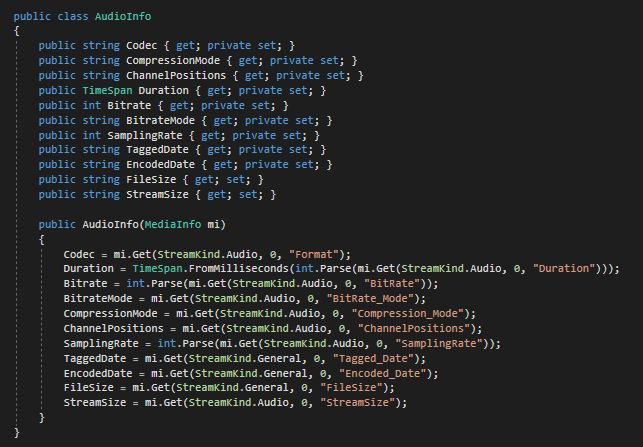
\includegraphics[width=17cm]{imgs/audio_extracting.jpg}
\end{center}\vspace{-0.3cm}
\caption[Extracting meta-data from audio files]{Extracting meta-data from audio files} \label{audio_extracting}
\end{figure}




\subsection{``Search for an operation'' Implementation}
\label{sub:search_for_an_operation_implementation}

Following the regisration of a new operation, the user can navigate to the home page, where they can search for an operation stored in the relational database. As mentioned in subsection \ref{sub:register_new_operation_implementation}, two methods with the same name were created in the HomeController, one for the HttpGet and one for the HttpPost request.


\subsection{``Operation Details'' Implementation}
\label{sub:operation_details_implentation}



\blindtext

\blindtext

\blindtext



\chapter{Testing}
\label{chapterlabel6}

% This just dumps some pseudolatin in so you can see some text in place.
\blindtext

\chapter{Conclusion and Project evaluation}
\label{chapterlabel7}

%waqas
This chapter completes the project by revising the project goals, objectives and personal aims in order to assess whether they were met. An evaluation of the project examines the processes and procedures that were implemented to develop and deliver the project. Finally, future work and and concluding remarks are presented.

\section{Project Goals}

The introductory goals of the project have been defined quite broadly on purpose since there was substantial uncertainty  in the initial stage of the project about how quickly the development of the application would proceed. The author is generally satisfied with the results, although some components were more successful than the rest. The first project goal was to develop and deliver a web application with a clear and usable interface that will enable the user to register and upload all the relevant information of an operation, including the generated from the operation media files. Sensor Fusion Web Application has been successfully deployed and tested at \url{https://sensorfusion.azurewebsites.net/} and all the aforementioned functionalities have been included. The second goal was to build the back-end part of the web application, that will make it able to extract all the meta-data from the selected media files, store the media files in a private file storage and store all the information of the operation in a relational database. That was arguably the hardest part of the application, but the application now fully supports the extraction,storing and retrieval of all the metadata related to the media files. The second goal was to develop a combination of front-end and back-end components that will allow the user to search for an operation stored in the relational database, apply certain filters to reduce the displayed results in order to find an operation of their choice. This goal has also been achieved, as the home page of the application demonstrates the listing and searching capabilities of the web application. The third and final goal of the application was to design a distinct web page in the application where the user is able to view all the aggregated information that is related to a specific operation. The web application includes a separate ``details'' page where the user can all the relevant information of an operation, including the media files' URL and metadata information. Overall, the author's opinion is that the development of the application went wery well. During the development process of the server side, there was never an occasion where where a part of the application had to be restructured or reconstructed in order to make another part of the application work properly, which by itself was a strong sign of separation of concerns.

\section{Fulfilment of Personal Aims}

The personal aims of this project were mostly focused on learning more and becoming proficient in building and developing dynamic web applications. In regards to the server side language, the programming language of choice was C\# and ASP.NET Core framework, as described throughout the current report. During the development phase and after the first weeks of learning C\# and ASP.NET, it was only able to build static pages and some basic database manipulation. Nonetheless, after a intense period, the author was able to realise the true potential of the framework and from then on the development stage progressed at a rapid pace. Overall, the learning experience was very intensive but at the same time very rewarding, and thus this particular stage can be regarded as one of the most significant personal achievements of the whole project. Feeling confident to develop robust web application in a new programming language like C\# and being able to build an application from scratch in the ASP.NET framework was certainly a fulfilment of one of my personal aims. By undertaking this particular project, the front-end programming skills of the author have been significantly improved. After the completion of the project, the author gained a significant amount of knowledge on creating attractive user interfaces and is comfortable to a certain level to understand the proper use of JavaScript and HTML5. Furthermore, the use of jQuery and Ajax methods helped with the development of a firm understanding of how JavaScript can be used in order to create a rich and interactive website. Finally, the last achieved personal aim was to build onn previous knowledge of MySQL database. By creating the web application, it provided the opportunity to further improve into a very advanced level the knowledge that had been gained through the GC04 and COMPGC06 database modules. The application helped develop and refine the skills needed to create arguable the most elaborate, robust and stable database schema explained in detail in Chapter \ref{chapterlabel3}.


\textbf{textHere}\\

\textbf{textHere}\\

\textbf{textHere}\\

\textbf{textHere}\\

\textbf{textHere}\\




\section{Critical Evaluation}


\section{Future Work}


\section{Conclusion}




\addcontentsline{toc}{chapter}{Appendices}

% The \appendix command resets the chapter counter, and changes the chapter numbering scheme to capital letters.
%\chapter{Appendices}
\appendix
\chapter{Source Code}
\label{app:source_code}

katherine hinke

\chapter{System Manual}
\label{app:system_manual}
 % description of document, e.g. type faces, TeX used, TeXmaker, packages and things used for figures. Like a computational details section.
% e.g. http://tex.stackexchange.com/questions/63468/what-is-best-way-to-mention-that-a-document-has-been-typeset-with-tex#63503

% Side note:
%http://tex.stackexchange.com/questions/1319/showcase-of-beautiful-typography-done-in-tex-friends 
% You could separate these out into different files if you have
%  particularly large appendices.

% This line manually adds the Bibliography to the table of contents.
% The fact that \include is the last thing before this ensures that it
% is on a clear page, and adding it like this means that it doesn't
% get a chapter or appendix number.
\addcontentsline{toc}{chapter}{Bibliography}

% Actually generates your bibliography.
\bibliographystyle{unsrt}
\bibliography{bibliography}

% All done. \o/
\end{document}
